\chapter{Methodology}

\section{Game Theory}
Here we will present some of the game theory concepts we use in our models, for more thoroughly explanation of game theory, see: \cite{nisan2007algorithmic}.
\subparagraph{One shot game}
This type of game assumes that players act at the same time instant, therefore there is no causality. A game in strategic (normal) form can be described by three elemetns:
\begin{itemize}
\item the set of players $i \in I$, which we take to be the finite set ${1,2,....,I}$.
\item the pure-strategy space $s_{i}\in S_{i}$ for each player i, where $s_{i}$ is a possible action of player i.
\item and payoff functions $U$, which gives the players utility functions for each profile $s=(s_{1},s_{2},...,s_{I})$ of strategies.
\end{itemize}
A general solution concept for games of economic interest is the Nash Equlibrium solution. A Nash Equilibrium is a profile of strategies such that each players strategy is an best response to the other players strategies. 
\subparagraph{Nash Equilibrium}
A pure strategy profile $s^{*}$ is a Nash eqilibirum if, for all players $i$
\begin{equation}
U_{i}(s^{*}_{i},s_{-i}^{*})\geq U_{i}(s_{i},s^{*}_{-i}) \in S_{i}
\end{equation}
\subparagraph{Stackelberg}
Also known as a leader-follower game, it introduces multiple stages. The leader commits itself first, chooses its strategy, then the followers respond sequentially. The Stackelberg model can be solved to find the subgame perfect Nash Equilibrium, i.e. the strategy profile that serves each player best, given the strategies of the other players and that entails every player playing in a Nash Equilibrium in every subgame.
\subparagraph{Subgame-perfect equilibrium}
A strategy profile $s$ is a subgame perfect equilibrium if it represents a Nash Equilibrium of every subgame of the original game.
\subparagraph{Socially optimal}
A socially optimal outcome is the set of choices that maximizes the sum of all players payoffs. 
\subparagraph{Price of stability}
The price of stability (PoS) of a network game, is the ratio between the maximum sum of the players payoff, in a stable outcome, and the Socially optimal outcome.
\section{Netlogo}
In addition to analyzing the different models with game theory, we created a simulator for the models, in a program called Netlogo. Netlogo is a programmable modeling environment for simulating natrual and social phenomena. It is well suited for modeling complex systems developing over time \cite{netlogo}.
Netlogo where good to model our complex network formation games, and at the same time provided us with a good graphical user interface, that enabled us to see the result of the games, and also to easily adjust the different parameters.
In Figure \ref{fig:netlogo} we see the user interface, which are used to setup the parameters, start the modeling, and showing the resulting network formation. Figure \ref{fig:netlogo-code} shows how the coding interface looked like. For detailed overview of the code used in our different models, see the appendix.
\begin{figure}[h]
\centering
  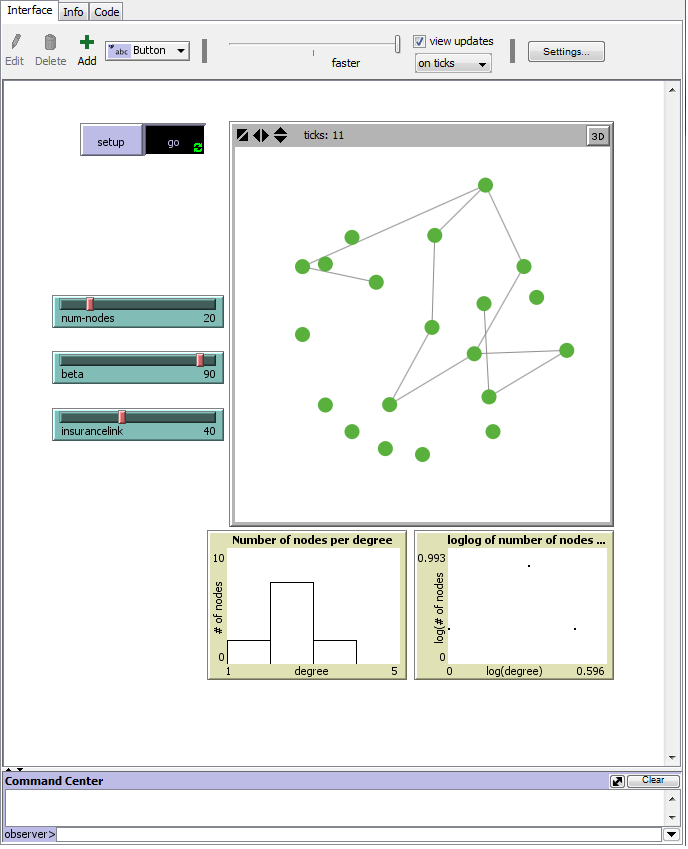
\includegraphics[width=0.9\linewidth]{../Figures/netlogoexample.png}
  \caption{\label{fig:netlogo} The figure shows a screen capture of netlogo, while we are running one of our simulations.}

\end{figure}
\begin{figure}[h]
\centering
  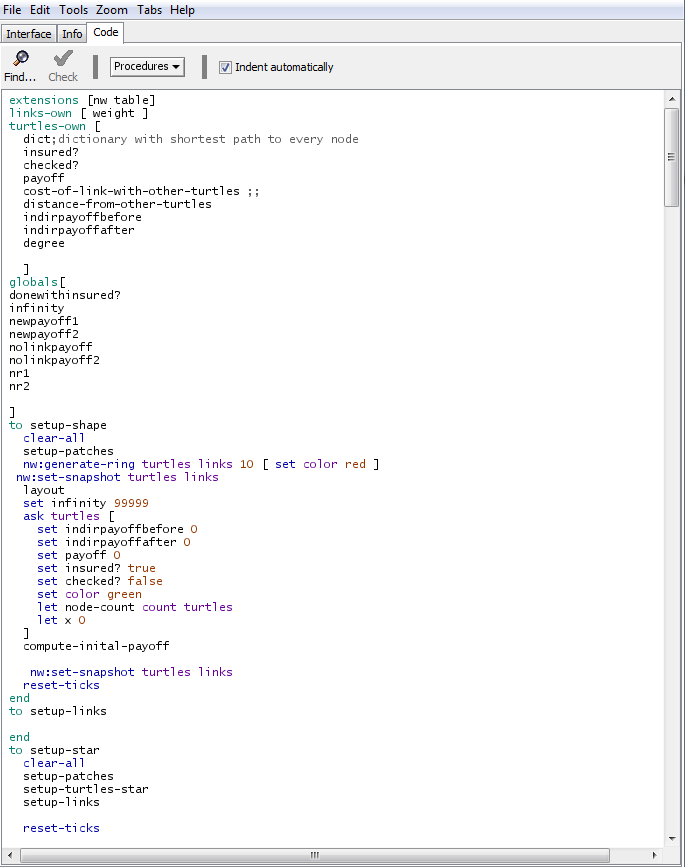
\includegraphics[width=0.9\linewidth]{../Figures/netlogocodeexample.png}
  \caption{\label{fig:netlogo-code} The figure shows how the code interface in netlogo looks like.}

\end{figure}
\subparagraph{Bayesian game}
In Bayesian games, information about the other players characteristics is incomplete. In these types of games, there are one player(the agent) who knows both types, and another player (the principal) who does not know the type of the other player. 

A pooling equilibrium, is a equilibrium where all both types of the agent chooses the same action, i.e. the principal is not able to distinguish the two types. 
A separating equilibrium is an equilibrium where the agents of different types, choose different actions, and thus the principal is able to determine the agents type by observing his actions.


